\section{Molekül- und Hybridorbitale}
\authors{Ali Serour, Johannes Wörsdörfer}
\subsection{Molekülorbitale}

Die Molekülorbitaltheorie ist eine Näherung zur quantenchemischen Beschreibung von Molekülen. Man nähert die Gesamtwellenfunktion mithilfe der Molekülorbitale an. Molekülorbitale sind Einteilchenwellenfunktionen beziehungsweise Linearkombinationen von Atomorbitalen $\chi_k$ (\ref{Linearkombination zweier Atomorbitale}):

\begin{equation}
 \label{Linearkombination zweier Atomorbitale}
 	\psi_i = \sum \limits_{k=1}^{n} c_{ik} \chi_k
\end{equation}

Dieses Verfahren wird LCAO (linear combination of atomic orbitals) genannt. Die Koeffizienten $c_{ik}$ geben an, wie stark die einzelnen Atomorbitale zu den jeweiligen Molekülorbitalen beitragen.
Es wird angenommen, dass eine chemische Bindung durch konstruktive Interferenz von Atomorbitalen beschrieben werden kann. Diese Interferenz führt zu bindenden Molekülorbitalen. Analog dazu resultieren antibindende Molekülorbitale aus destruktiver Interferenz der Atomorbitalbasis (siehe Abbildung \ref{fig:LCAO}). Die Energie bindender MOs ist niedriger als die antibindender \cite{Reinhold}.

\begin{dsafigure}
  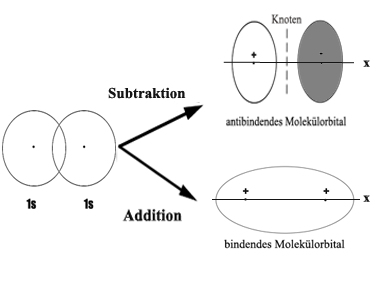
\includegraphics[width=\columnwidth]{LCAO3.png}
  \caption{Links: Linearkombination von 1$s$-Orbitalen zu $\sigma$-Molekülorbitalen. Unten rechts: Linearkombination der Atomorbitale, die zu einem bindenden Molekülorbital führt. Oben rechts: Linearkombination der Atomorbitale, die zu einem antibindenden Molekülorbital führt. }
  \label{fig:LCAO}
\end{dsafigure}

Zur Veranschaulichung bedienen wir uns des Molekülorbital-Diagramms des Wasserstoffmoleküls (siehe Abbildung \ref{fig:MO-Diagramm}).
Die beiden 1$s$-Atomorbitale der Wasserstoffatome bilden ein bindendes und ein antibindendes Molekülorbital. Die Anzahl der Molekülorbitale entspricht immer der Anzahl der Atomorbitale. Beim Besetzen der Molekülorbitale mit Elektronen werden die selben Regeln eingehalten wie im Falle von Atomorbitalen (Aufbauprinzip, Pauli-Verbot, Hundsche Regel). Die Bindungsordnung (BO) lässt sich mit der Formel
\begin{equation}
 \label{Bindungsordnung}
 	BO = \frac{n_b-n_a}{2}
\end{equation}

darstellen, wobei $n_b$ die Zahl der Elektronen in bindenden und $n_a$ die Zahl der Elektronen in antibindenden Orbitalen bezeichnet. Für das Wasserstoffmolekül ergibt sich demzufolge: $(2-0)/(2) = 1$. Somit sind die beiden Wasserstoffatome durch eine Einfachbindung gebunden.

 \begin{dsafigure}
  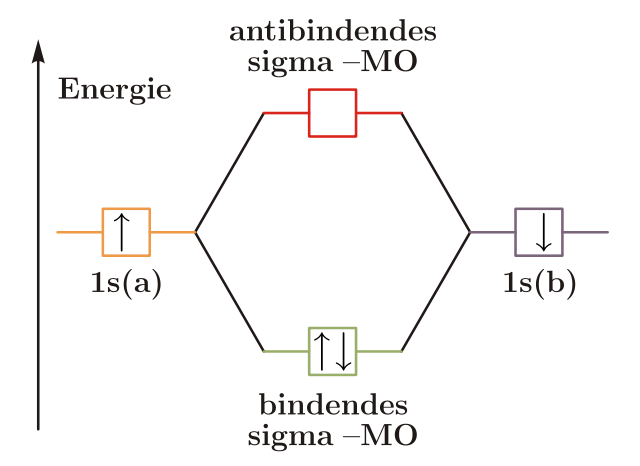
\includegraphics[width=\columnwidth]{MO-Diagramm.png}
  \caption{Molekülorbital-Diagramm des Wasserstoffmoleküls \cite{WasserstoffMO}.}
  \label{fig:MO-Diagramm}
\end{dsafigure}

Diese Einfachbindung wird als $\sigma$-Bindung bezeichnet. $\sigma$-Bindungen beziehungsweise $\sigma$-Orbitale sind rotationsymmetrisch. Das heißt, sie ändern sich durch eine Rotation um die Bindungsachse nicht (siehe Abbildung \ref{fig:LCAO}). Neben den $\sigma$-Bindungen gibt es auch $\pi$-Bindungen. Diese Bindungen beziehungsweise Orbitale sind nicht rotationssymmetrisch. Eine Rotation um 180$^\circ$ um die Bindungsachse ändert ihr Vorzeichen.

\subsection{Hybridorbitale}

Eine alternative Beschreibung der Bindungsverhältnisse bieten die Hybridorbitale. Sie können ohne großen Recheneinsatz ermittelt werden und geben ein einfaches, qualitatives Bild.
Methan hat die Form eines Tetraeders, in dem alle Wasserstoffatome den gleichen Abstand vom Kohlenstoffatom aufweisen \cite{Riedel04}. Kohlenstoff hat die Elektronenkonfiguration $2s^2 2p^2$. In der Hybridorbital-Beschreibung wird das $s$-Orbital mit den drei $p$-Orbitalen linear kombiniert, wobei vier tetraedrisch angeordnete $sp^3$-Hybridorbitale entstehen (siehe Abbildung \ref{fig:Methan}).
Die tetraedrische Geometrie des Methanmoleküls wird erzeugt, indem die 1$s$-Orbitale der Wasserstoffatome mit den $sp^3$-Hybridorbitale konstruktiv interferieren. Jedoch sind die Energien der Orbitale in diesem Modell im Gegensatz zur Molekülorbitaltheorie (siehe Abbildung \ref{fig:MO-Diagramm}) nicht definiert. 



 \begin{dsafigure}
  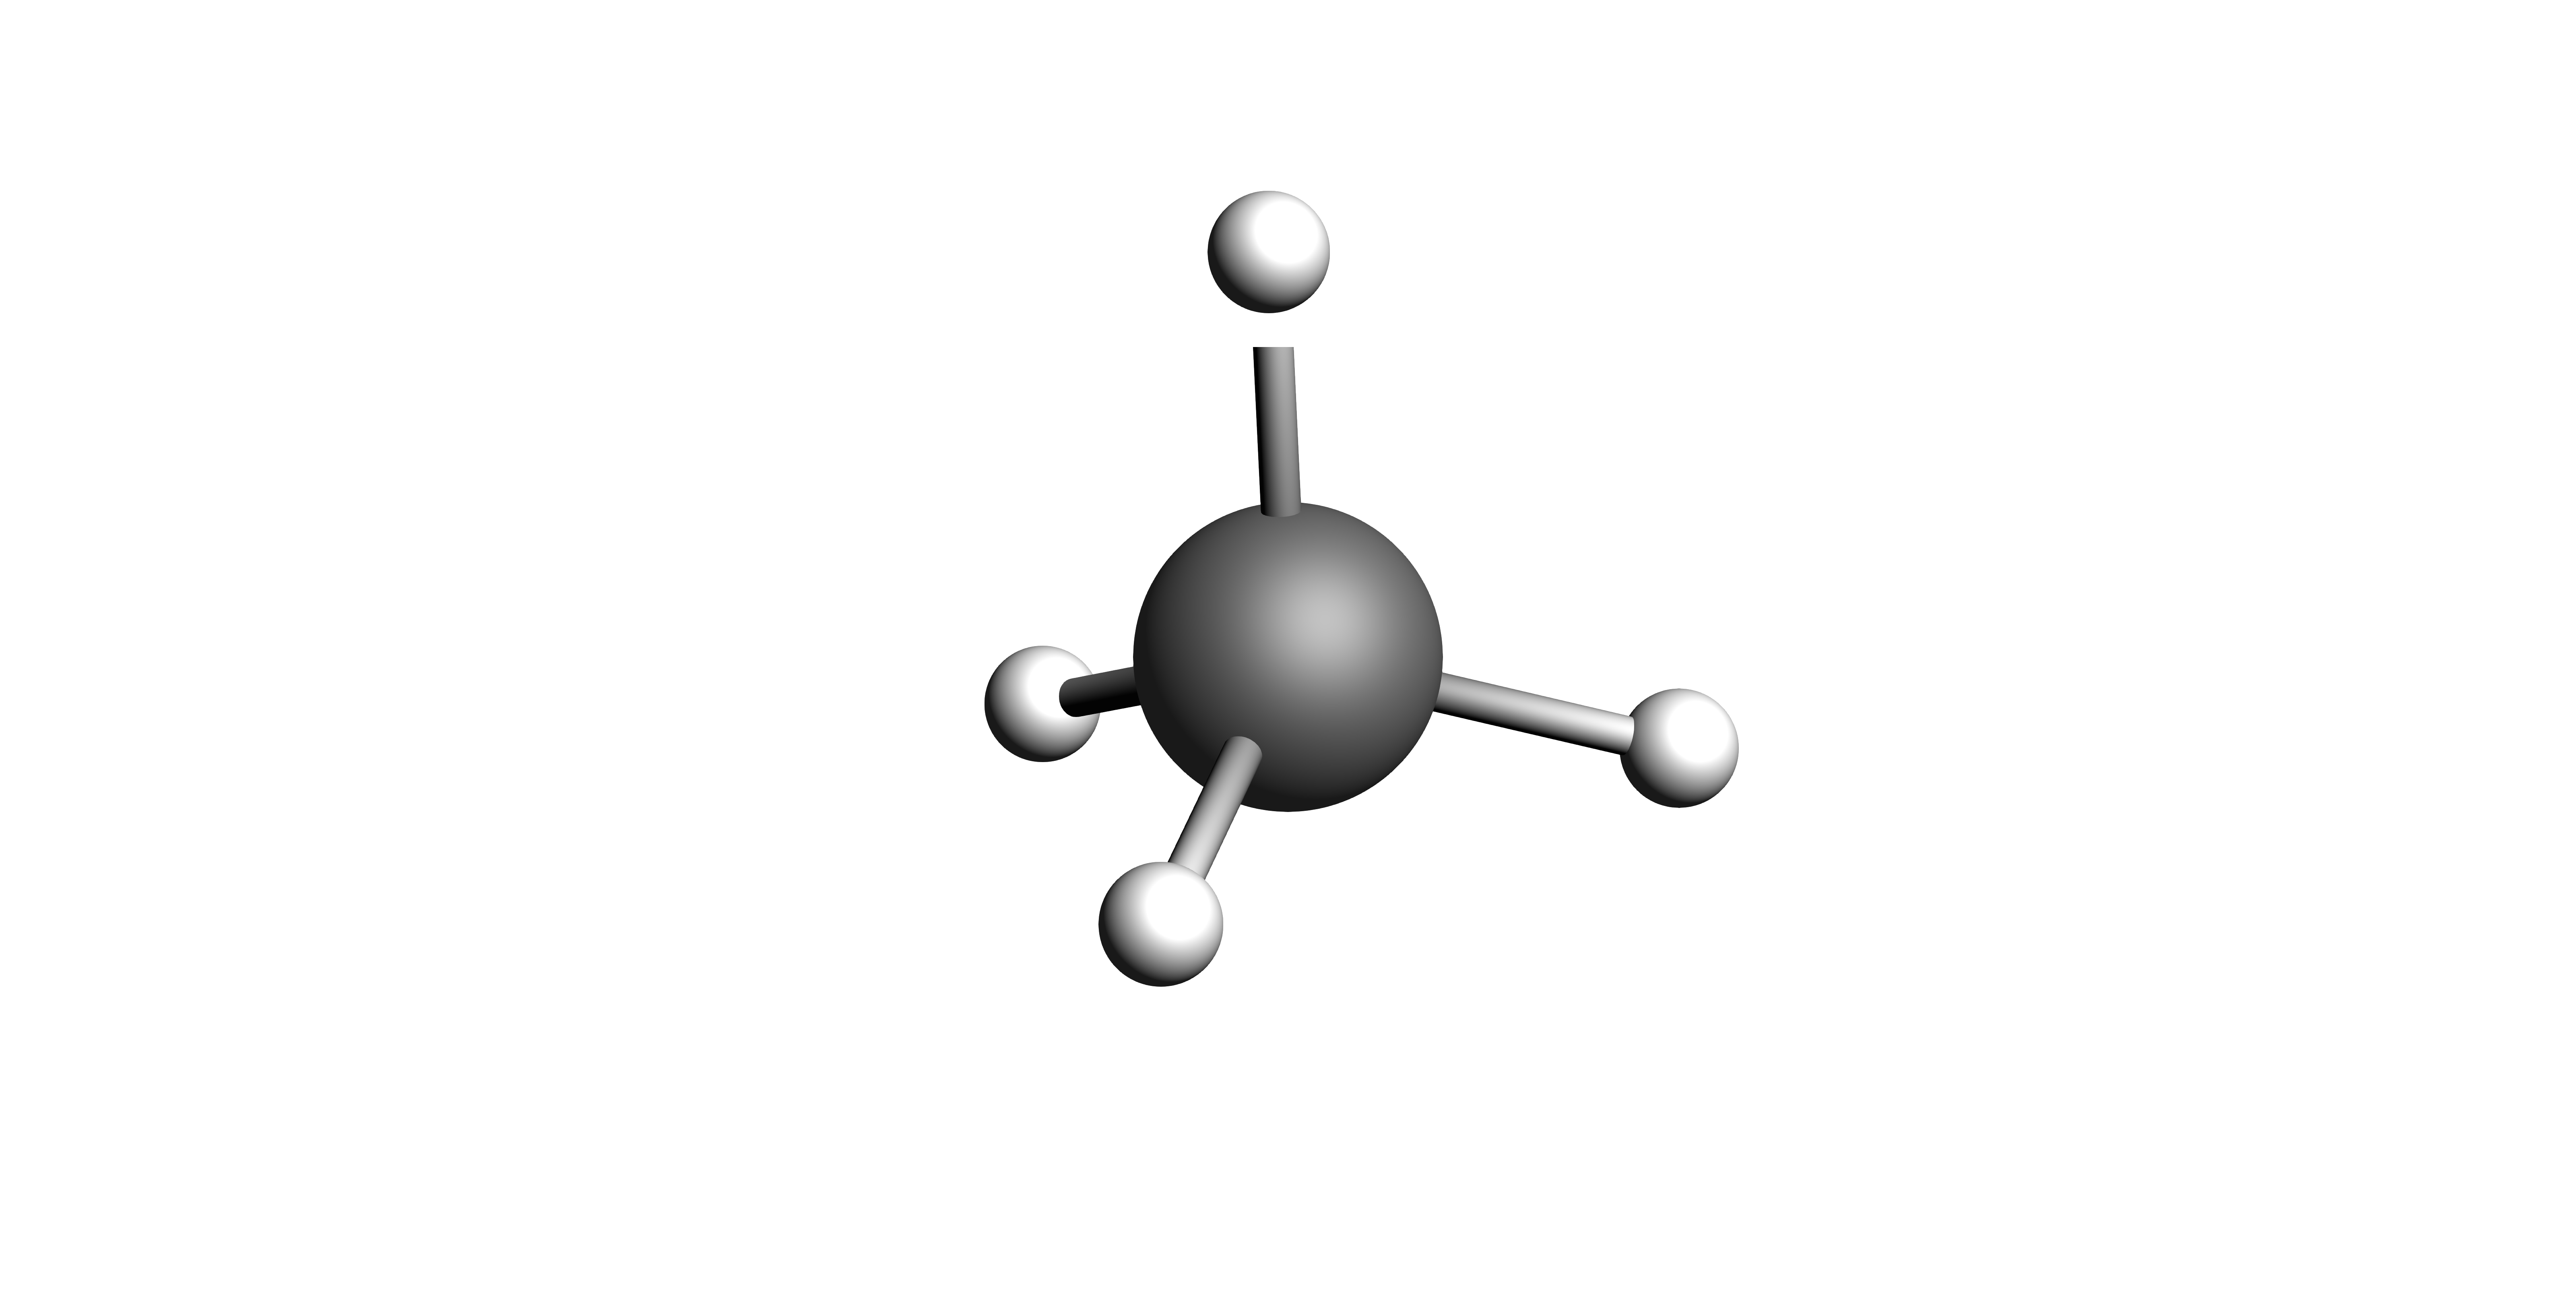
\includegraphics[width=\columnwidth]{Methan.jpg}
  \caption{3D-Modell des Methans \cite{ADF2017authors}. }
  \label{fig:Methan}
\end{dsafigure}

Des Weiteren führen die Linearkombinationen von einem $s$-Orbital und zwei $p$-Orbitalen zu drei $sp^2$-Hybridorbitalen, mit denen man die Bindungsverhältnisse im Ethen beschreiben kann. Außerdem führt eine Linearkombination von einem $s$-Orbital und einem $p$-Orbital zu zwei $sp$-Hybridorbitalen, mit denen man die Bindungsverhältnisse im Ethin beschreiben kann.
